\chapter{Evaluation}\label{appendix_evaluation}

\FloatBarrier
\section{Survey Questions}

\begin{figure}[h!]
	\centering
	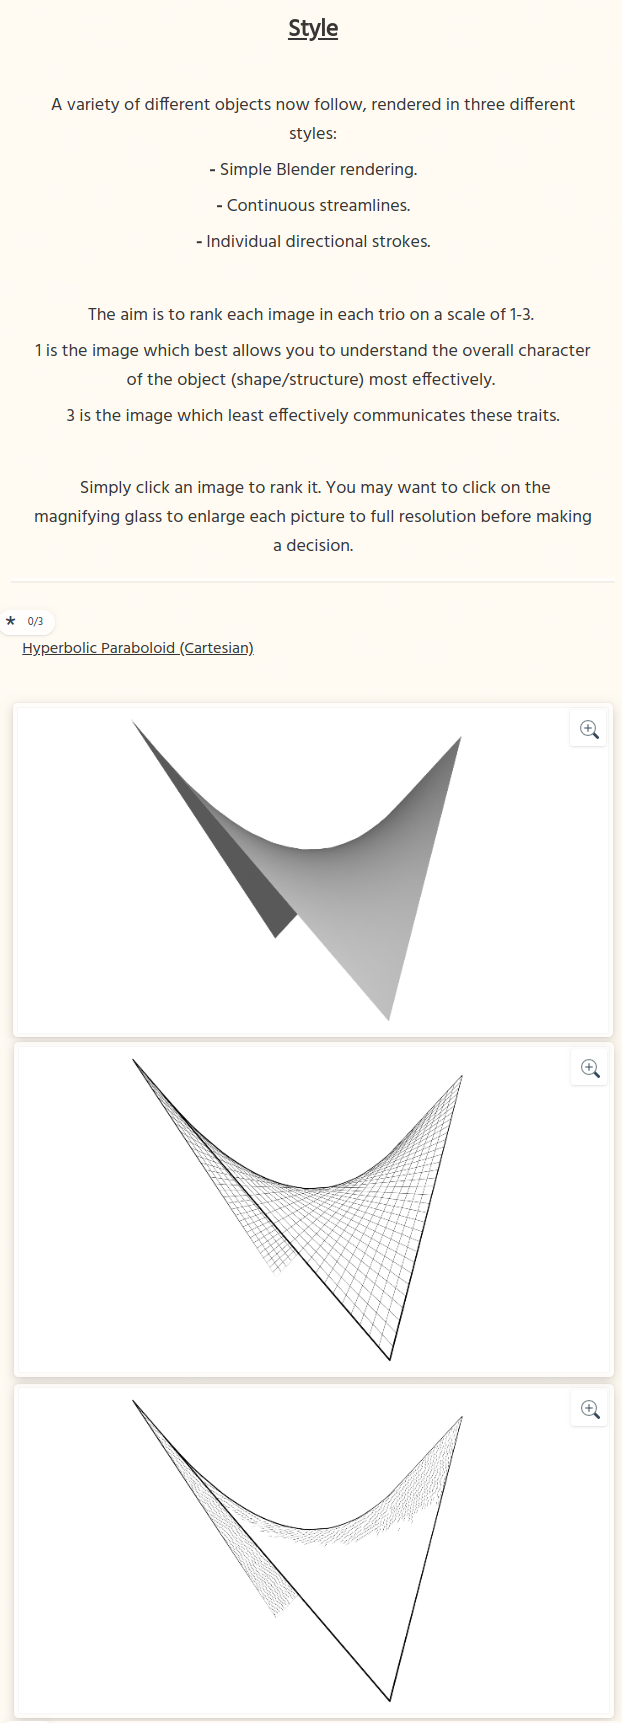
\includegraphics[height=0.8\textheight]{images/eval_styles.png}
	\caption{Style evaluation sample question. This question was repeated with a further 12 objects, covering a mixture of mathematical surfaces and assorted objects.}\label{eval_styles}
\end{figure}

\begin{figure}[h!]
	\centering
	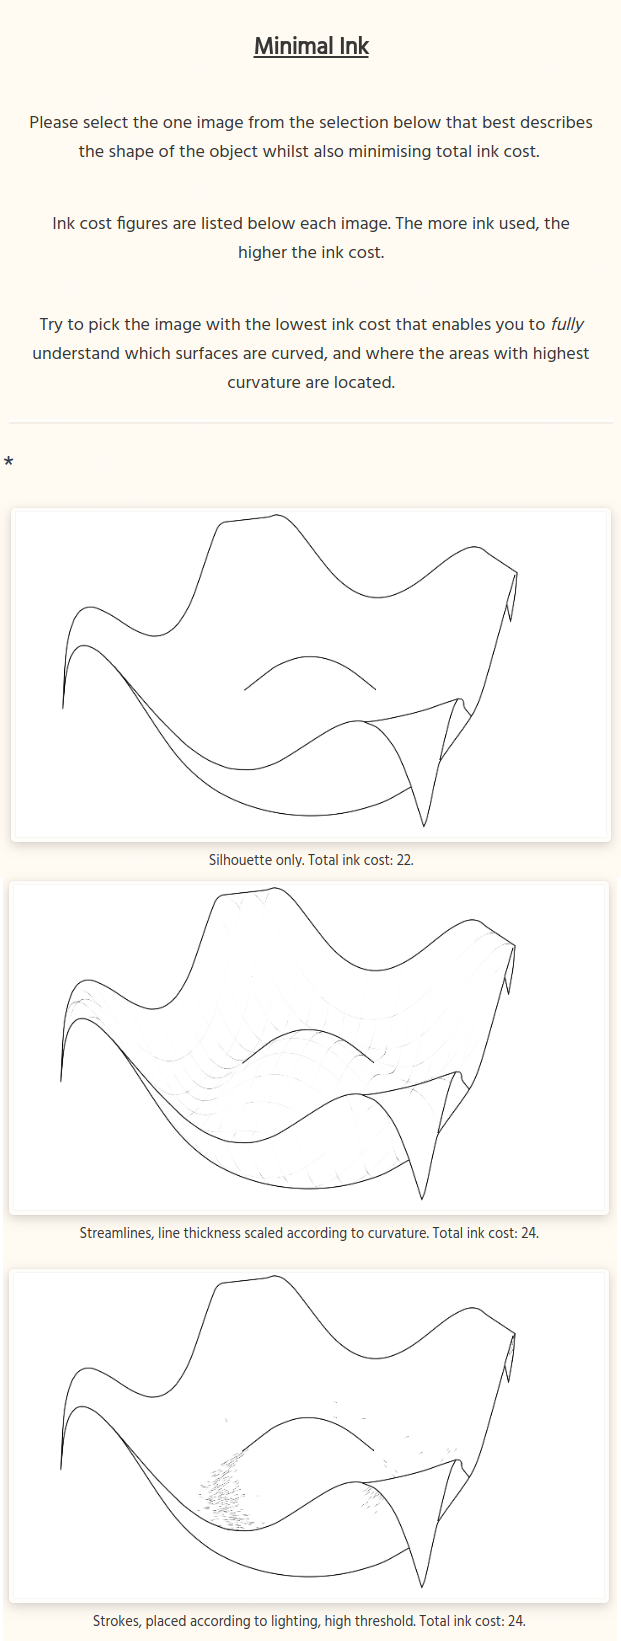
\includegraphics[height=0.8\textheight]{images/eval_ink_1.png}
	\caption{Parsimony of ink evaluation question (partial).}\label{eval_ink_1}
\end{figure}

\begin{figure}[h!]
	\centering
	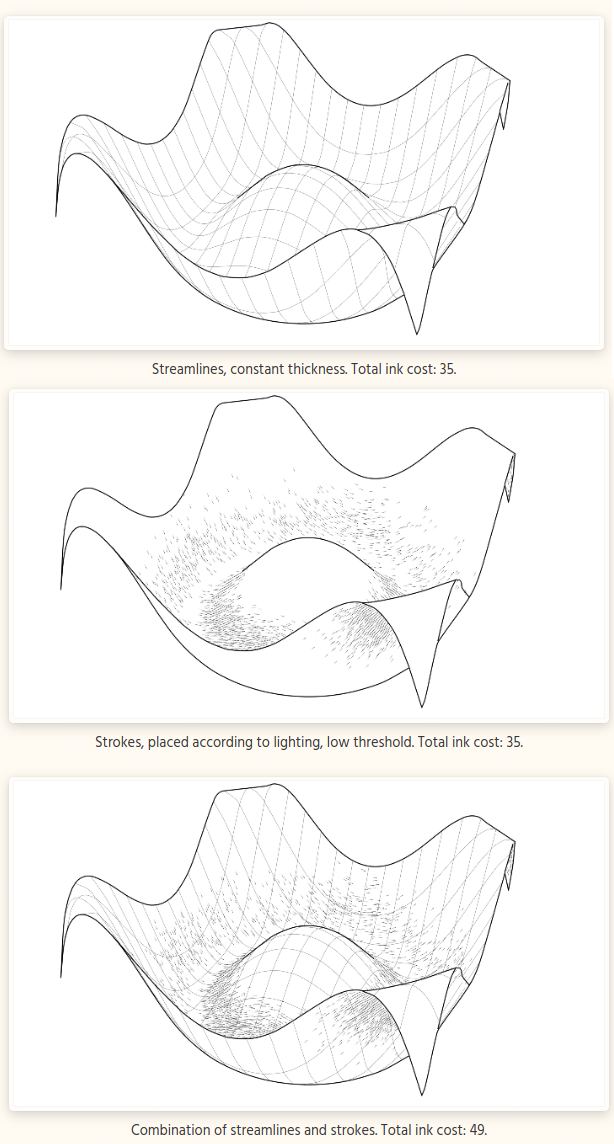
\includegraphics[height=0.8\textheight]{images/eval_ink_2.png}
	\caption{Parsimony of ink evaluation question (continued).}\label{eval_ink_2}
\end{figure}

\begin{figure}[h!]
	\centering
	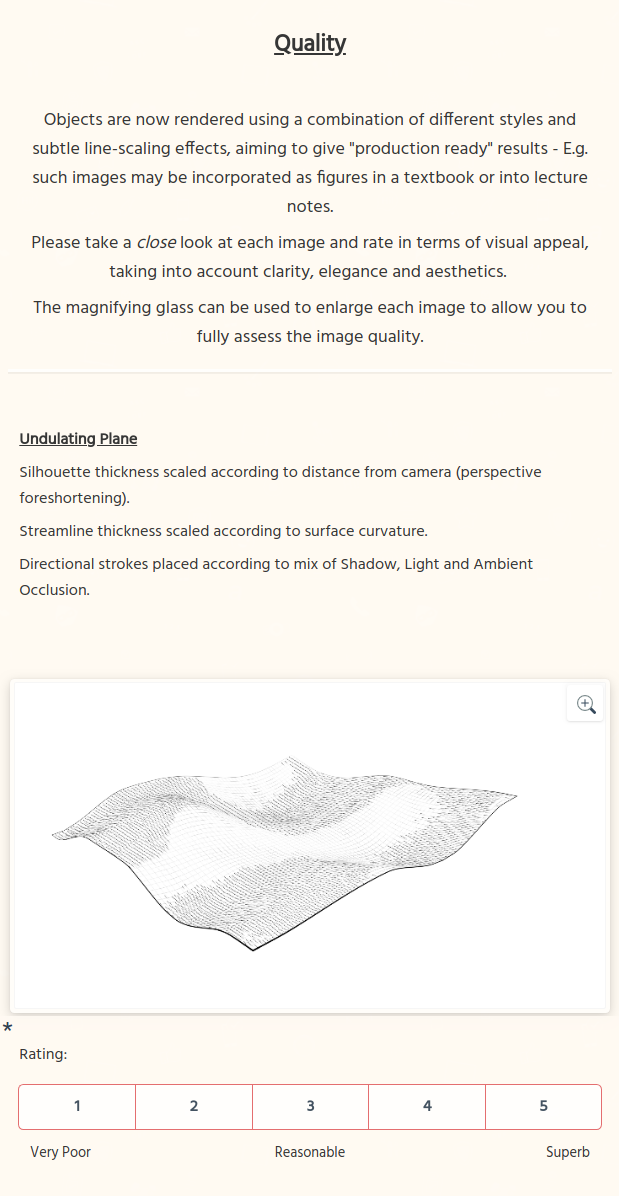
\includegraphics[height=0.8\textheight]{images/eval_quality.png}
	\caption{Quality evaluation sample question. This question was repeated with a further 10 objects, covering a mixture of high-quality mathematical surfaces and assorted objects.}\label{eval_quality}
\end{figure}

\FloatBarrier
\section{Survey Results}\label{appendix_eval_results}

\begin{figure}[h!]
	\centering
	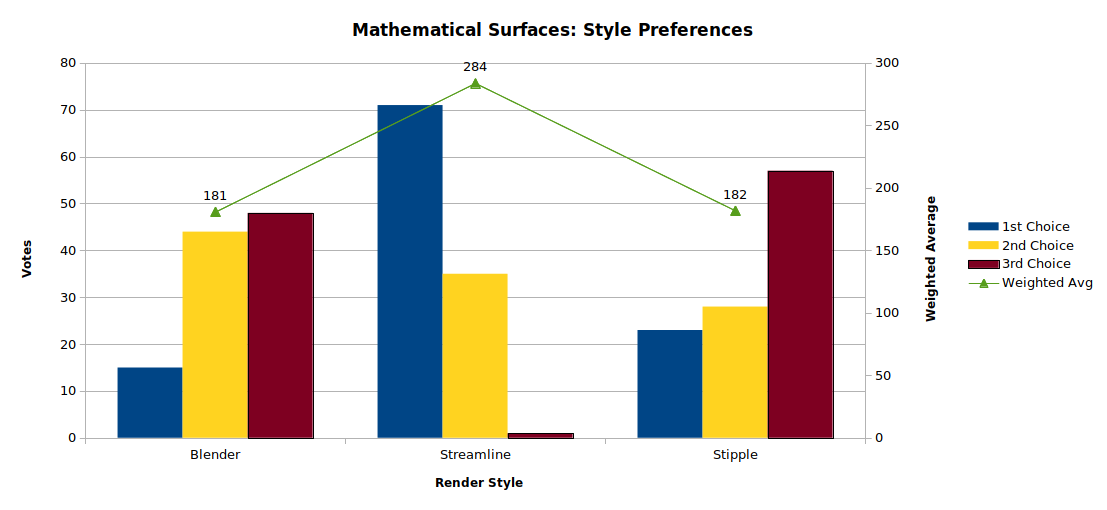
\includegraphics[width=\textwidth]{images/eval_chart_styles_math.png}
	\caption{Style preferences for mathematical surfaces. Bars represent the sum of votes across all presented images. Weighted average is computed with a weight of 3 applied to 1st choices, 2 applied to 2nd choices and 1 applied to 3rd choices. Results show strong preference for the streamline style, followed by roughly equal preference for Blender and stipple styles.}\label{eval_chart_styles_math}
\end{figure}

\begin{figure}[h!]
	\centering
	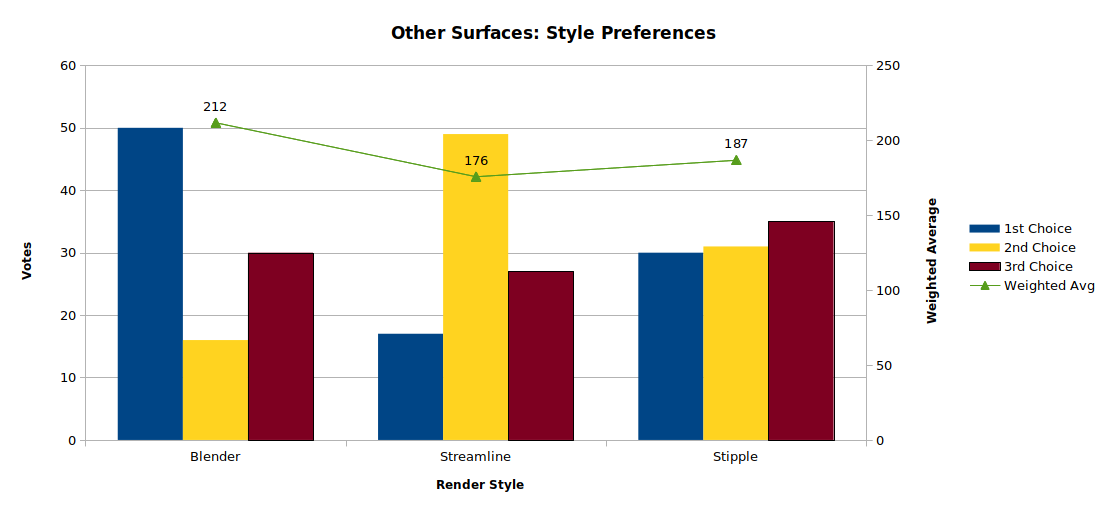
\includegraphics[width=\textwidth]{images/eval_chart_styles_other.png}
	\caption{As Figure \ref{eval_chart_styles_math}, but with consideration to non-mathematical surfaces. Results show moderate preference for Blender style, followed by roughly equivalent preferences for implemented NPR styles.}\label{eval_chart_styles_other}
\end{figure}

\begin{figure}[h!]
	\centering
	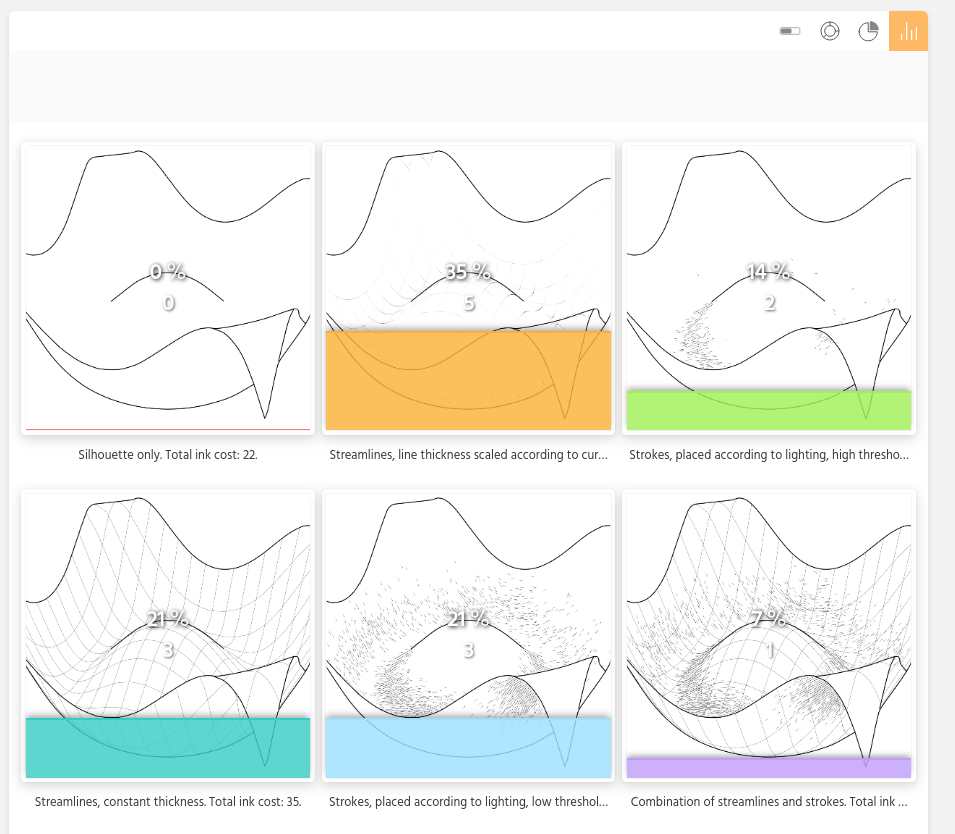
\includegraphics[width=\textwidth]{images/eval_ink.png}
	\caption{Results showing number of votes for each image. Top centre is most-voted, suggesting structure can be communicated well with only minimal ink, using streamlines scaled according to curvature.}\label{eval_ink}
\end{figure}